\section{Client}
L'applicazione lato client viene sviluppata con il linguaggio di programmazione python, utilizzando l'insieme di moduli Pygame 
per la realizzazione dell'interfaccia grafica. (Ulteriori informazioni su pygame al link \href{https://www.pygame.org/}{https://www.pygame.org/})
\\\\Nel codice viene implementata la logica per garantire le funzionalità dell'applicazione, come l'interfaccia grafica, l'acquisizione 
dei dati dei sensori derivanti dal cloud, il cambiamento di stato e l'acquisizione degli input dell'utente.\\\\
Lo stato corrente viene mantenuto da specifiche variabili di stato, che vengono modificate nel momento in cui si verificano eventi gestiti dai moduli pygame
(interazione del mouse con un pulsante presente sullo schermo). Inoltre, vengono mantenute ulteriori informazioni sui dati dell'applicazione in precise variabili:
\begin{verbatim}
roll_state = False      # variabile di stato corrente
dice_quantity = 1       # numero di dadi da lanciare
dice_state = []         # stato dei dadi usciti: es [6, 3, 1]
dice_generate = False   # lancia la funzione di generaz dadi
result = 0              # risultato finale
\end{verbatim}
Nel complesso, il client realizzato permette di gestire la comunicazione bilaterale di dati tra il cloud e il microcontrollore, sfruttando
il protocollo di comunicazione LoRa. Le funzioni che permettono la connessione del client con il cloud sono definite dal protocollo 
di messaggistica MQTT, progettato esclusivamente per fini legati all IoT.
Di seguito si riportano brevemente le implementazioni software che riguardano la gestione della comunicazione
\textbf{uplink} e \textbf{downlink}.

\subsection{Gestione Uplink}
La gestione della comunicazione dei dati dal uC al cloud (e di conseguenza client) lato software viene gestita attraverso la funzione di callback 
\textit{on\_message()}, richiamata ad ogni nuovo messaggio ricevuto dall'applicazione lato cloud. Partendo dal presupposto che il payload ricevuto
dipende dallo stato corrente dell'applicazione, nella funzione di callback viene implementata la logica per l'elaborazione dei dati inviati dall' uC in base al valore
della variabile di stato \textit{roll\_state}. Successivamente viene poi convertito il payload ricevuto in stringhe leggibili e stampato il valore della variabili, 
dopo i dovuti shift eseguiti sull'array contenente il payload, per ottenere correttamente i dati.
\\\\Di seguito si riporta l'esempio per l'acquisizione della coordinata y dell'accelerazione dal payload dati ricevuto in cloud e la sua 
successiva elaborazione, per cambiare lo stato corrente del sistema:\\\\
\begin{verbatim}
if roll_state == True:
    gyr_y = (((((message_bytes[1] << 24) | message_bytes[2] << 16)
     | message_bytes[3] << 8) | message_bytes[4] ) & 0xFFFFFFFF)  

    if gyr_y & 0x80000000:
        gyr_y = gyr_y - 0x100000000
        print("gy: " + str(gyr_y) + "dice_generate: ", dice_generate)
        if abs(gyr_y) > 40000:
            dice_generate = True
\end{verbatim}
I passaggi illustrati vengono analogamente replicati per l'acquisizione dei dati (\textit{acc\_x, acc\_y}) relativi all'inclinazione della scheda
quando \textit{roll\_state = False}, ovvero quando il sistema è nella modalità di scelta dei dadi.
\\\\Si può quindi affermare che la comunicazione uplink viene gestita interamente nella funzione asincrona di callback, ma ha influenza 
sullo stato corrente del sistema e quindi anche sulla visualizzazione grafica dell'interfaccia utente e sulla comunicazione downlink.

\subsection{Gestione Downlink}
La gestione della comunicazione di dati dal client python al uC (passando per il cloud), è invece implementata nel ciclo infinito \textit{while True} 
del programma, dove sono presenti anche le funzioni di pygame per l'implementazione grafica dell'interfaccia utente.
\\\\Lo stato corrente può essere cambiato in qualsialsi momento dall'utente che interagisce con il client, premendo con il mouse sul pulsante
apposito contrassegnato con "Change mode". Nel momento in cui si rileva questo evento, viene generato il payload corrispondente allo stato che viene 
scelto dall'utente e successivamente inviato al cloud, in attesa che il microcontrollore lo riceva.
\\\\Di seguito è riportata la parte di codice in cui viene creato e inviato il payload al cloud per la comunicazione downlink:
\begin{verbatim}
if event.type == pygame.MOUSEBUTTONDOWN:
    if changeState_button.collidepoint(pygame.mouse.get_pos()):
        roll_state = not roll_state

        if roll_state == False:
            payload[0] = 0
            downlinks["downlinks"][0]["frm_payload"] = 
                base64.b64encode(payload).decode('utf8')
        else:
            payload[0] = 1
            downlinks["downlinks"][0]["frm_payload"] = 
                base64.b64encode(payload).decode('utf8')
        print("\r\n" + str(downlinks) + "\r\n")

        topic = "v3/" + CFG_APP_ID_AT_TTN + "/devices/" + 
            CFG_DEVICE_ID + "/down/push"
        client.publish(topic, json.dumps(downlinks))
\end{verbatim}
Come è possibile vedere dal codice, il payload da inviare al cloud viene organizzato nella struttura dati \textit{downlinks} e successivamente trasformato in un json
formattato in modo preciso per soddisfare la formattazione standard di un topic di tipo MQTT.\\\\
NOTA: Si è scelto di implementare la logica della comunicazione downlink in un ciclo temporizzato per 60 fotogrammi al secondo per esigenza di 
visualizzare in tempo reale i cambiamenti di stato nell'interfaccia grafica. Un'idea di ottimizzazione del progetto potrebbe essere
quella di svincolare i messaggi verso il cloud relativi al cambiamento di stato dalla grafica e quindi ridurre la frequenza con cui questi possono essere potenzialmente
inviati al cloud, dal momento che la frequenza di lettura dei dati del microcontrollore si aggira intorno a pochi secondi, non così frequente come il ciclo di aggiornamento della grafica.


\subsection{Interfaccia grafica}
L'interfaccia grafica viene implementata utilizzando i moduli per la generazione di elementi grafici messi a disposizione da pygame.
La scelta stilistica di utilizzare pygame è giustificata dalla necessità di rendere l'esperienza dell'utente più intuitiva possibile.
L'interfaccia grafica è realizzata in modo dinamico, per fare in modo che al cambiamento di stato del sistema, si modifichi in tempo reale.
\\\\La grafica realizzata presenta un pulsante per poter passare dallo stato di scelta dei dadi allo stato di lancio e un pulsante per resettare il risultato
e ritornare nella situazione iniziale, necessario per poter effettuare un nuovo lancio una volta ottenuto un risultato.
\\\\Di seguito è riportato un esempio dell'interfaccia grafica realizzata con le funzioni di pygame, in cui si mostra il risultato di un lancio dei dadi:
\begin{figure}[H]
    \centering
    \fbox{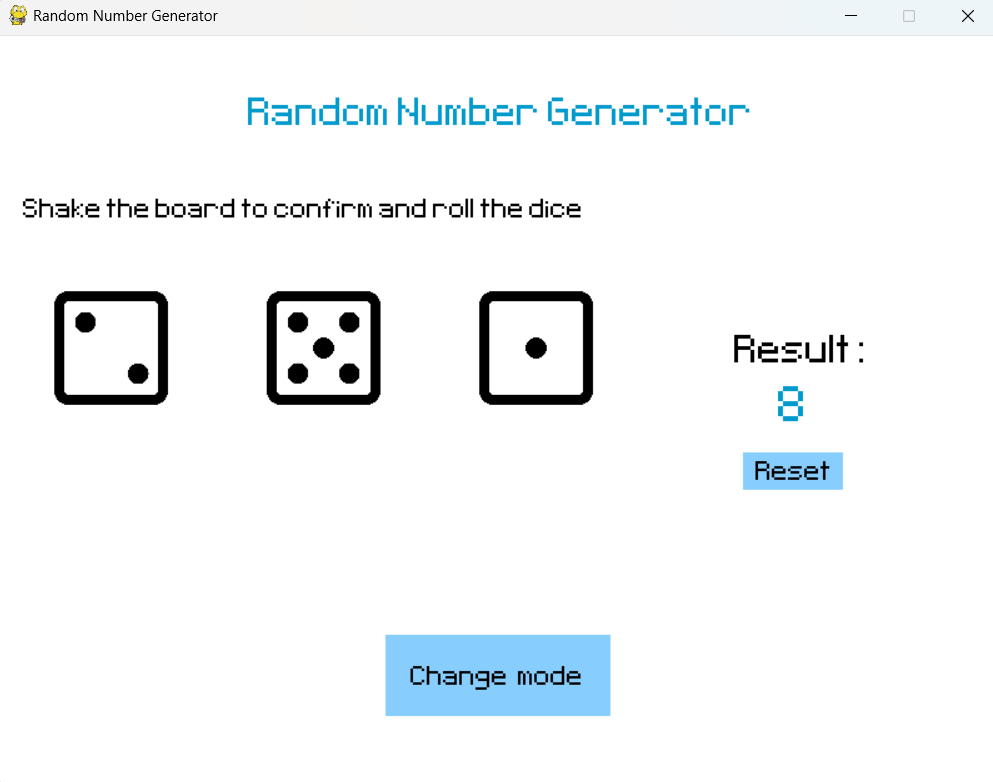
\includegraphics[width=0.7\textwidth]{RollStateON3.png}}
    \caption{Interfaccia grafica dell'applicazione}
    \label{fig:RollStateON3}
\end{figure}
Entrando nei dettagli della struttura del codice, l'interfaccia viene aggiornata con un massimo di 60 fotogrammi al secondo dalla funzione:
\begin{verbatim}
clock.tick(60)
\end{verbatim}
In ciascuno di questi fotogrammi vengono generati gli elementi grafici attraverso le apposite funzioni di pygame:
\begin{itemize}
    \item \Verb#pygame.draw.rect()# per disegnare sullo schermo gli oggetti di tipo Rect precedentemente creati (bottoni)
    \item \Verb#screen.blit()# per disporre sullo schermo i testi creati in precedenza. (screen è l'oggetto che identifica lo schermo)
\end{itemize}
Ad ogni fotogramma viene inoltre implementata una logica per la disposizione corretta dei dadi nello spazio, dipendente dal numero di dadi attualmente
selezionati per il lancio espressi nella variabile \textit{dice\_quantity}. Per garantire una disposizione simmetrica dei dadi si immagina di
suddividere lo spazio in una matrice 2 righe e 3 colonne da cui, con precise formule matematiche si può ricavare la coordinata precisa di generazione di ciascun dado:
\begin{verbatim}
for i in range(0, dice_quantity):
    n_cols = 3
    dice_x = 40 + (i % n_cols)*170 # 40 = x di partenza + 
        (100 + 70 = dimensione dado + spazio tra i dadi)
    dice_y = 200 + (i // n_cols)*120
    if dice_state == []:
        screen.blit(dice_surfaces[0], (dice_x, dice_y))
    else:
        screen.blit(dice_surfaces[dice_state[i]], (dice_x, dice_y))
\end{verbatim}
Nell'interfaccia grafica non vengono volutamente riportati i dettagli che riguardano la comunicazione tra il cloud e il client, ma solamente le funzionalità
indispensabili per una buona esperienza utente. 



















